\chapter{Program Representation}
\vspace{2cm}

\noindent
At this stage, we assume that we have successfully translated the functional
program into a lambda expression. In the next few chapters we will show how
to execute the program, reducing the lambda expression to normal form.

First of all we have to establish some \textit{representation} for the lambda
expression, as it is held in the computer’s memory. This chapter outlines the
possibilities.

\section{Abstract Syntax Trees}

In all implementations of graph reduction, the expression to be evaluated is
held in the machine in the form of its \textit{syntax tree}.

The leaves of the tree are constant values (such as 0, \ml{'a'}, \ml{TRUE}), built-in
functions (such as \ml{+}, \ml{$-$}, \ml{$\ast$}), or variable names.

The application of a function \ml{f} to an argument \ml{x} is represented thus:
\begin{center}
    \begin{forest}
        [\ml{@}
        [\ml{f}]
        [\ml{x}]
        ]
    \end{forest}
\end{center}
The `\ml{@}' sign is called the \textit{tag} of the node, and indicates that the node is an
application. We deal with functions of several arguments by currying:
\begin{center}
    \begin{forest}
        [\ml{@}
        [\ml{@}
        [\ml{+}]
        [\ml{4}]
        ]
        [\ml{2}]
        ]
    \end{forest}
\end{center}
This tree denotes the expression \ml{(+ 4 2)}, which shows the function \ml{+} applied
to the argument \ml{4}, giving a function \ml{(+ 4)}, which is then applied to the
argument \ml{2}. Figure 10.1 shows a slightly more complicated example.

\boxedfigure{
    \centering
    \begin{forest}
        [\ml{@}
            [\ml{@}
                [\ml{+}]
                [\ml{3}]
            ]
            [\ml{@}
                [\ml{@}
                    [\ml{$\ast$}]
                    [\ml{2}]
                ]
                [\ml{8}]
            ]
        ]
    \end{forest}
}{The tree of \ml{(+ 3 ($\ast$ 2 8))}}

A lambda abstraction (\ml{\tlb{x}body}) is represented thus:
\begin{center}
    \begin{forest}
        [\ml{\tl{x}}
        [\ml{body}]
        ]
    \end{forest}
\end{center}
The \ml{\tl{x}} tells that the node is a lambda abstraction and gives the formal
parameter.

The graph of the expression \ml{(CONS E$_1$ E$_2$)} will look like this
\begin{center}
    \begin{forest}
        [\ml{@}
        [\ml{@}
        [\ml{CONS}]
        [\ml{E$_1$}]
        ]
        [\ml{E$_2$}]
        ]
    \end{forest}
\end{center}
(\ml{E$_1$} and \ml{E$_2$} stand for arbitrary expressions, as usual.) The result of evaluating it
will be a \ml{CONS} cell, which we depict like this:
\begin{center}
    \begin{forest}
        [\ml{:}
        [\ml{E$_1$}]
        [\ml{E$_2$}]
        ]
    \end{forest}
\end{center}
where the `\ml{:}' tag labels the node as a \ml{CONS} cell (just as \ml{@} labels a node as an
application).

\section{The Graph}

The process of reduction performs successive transformations on the syntax
tree. During this process the \textit{tree} becomes a \textit{graph}, for reasons that will
become clear in Chapter 12. We use the term `graph' here in the sense of
`network', a collection of \textit{nodes} connected together by some \textit{directed edges}.
Figure 10.2 shows an example graph.

\boxedfigure{
    \centering
    \vspace{-10pt}
    \includegraphics[width=0.6\textwidth]{chapters/Fig10_2}
    \vspace{-10pt}
}{An example graph}

A graph differs from a tree in that two edges can point to the same node.
For example, in Figure~10.2 node D is a descendant of nodes A and C (we say
that it is \textit{shared}). A graph is said to be \textit{acyclic} if there is no path from a node
back to itself (Figure~10.2 is \textit{not} acyclic, since there is a path from node A to
itself, via node C). A directed acyclic graph is often abbreviated DAG.

\section{Concrete Representations of the Graph}

The pictures we have shown are still somewhat abstract. In a typical
implementation each node of the tree would be represented by a small
contiguous area of store, called a \textit{cell}. A cell holds a \textit{tag} which tells the type of
the cell (application, number, built-in operator, lambda abstraction, CONS
cell, etc.), and two or more \textit{fields}. The number of fields in a cell varies between
implementations. Many implement fixed-size cells with two fields, but some
have variable-sized cells. This issue is further discussed below. We may draw a
cell thus:
\begin{center}
    {%
        % Local changes: only apply inside this group
        \setlength{\tabcolsep}{16pt}   % horizontal padding
        \renewcommand{\arraystretch}{1.75} % vertical padding
       	\sffamily
        \footnotesize
        \begin{tabular}{|c|c|c|}
            \hline
            Tag & Field 1 & Field 2 \\
            \hline
        \end{tabular}
    }%
\end{center}

A field may contain the address of another cell, in which case we say that it
is a \textit{pointer}, and that it \textit{points to} the cell. We draw a pointer field like this:
\begin{center}
    {%
        \sffamily
        \footnotesize
        %
        \begin{tikzpicture}
            \node[draw, rectangle, minimum width=3cm, minimum height=0.75cm] (address) at (0,0) {Address\phantom{XXXX}};
            \node (cell) at (3.5,0) {\normalfont\normalsize Another cell};
            \draw[-{Stealth[length=3mm,width=2mm]}, thick] ([xshift=0.5cm]address.center) -- (cell.west);
        \end{tikzpicture}
    }%
\end{center}

Alternatively, a field may contain an \textit{atomic} (non-pointer) data value. We
draw a non-pointer field like this:
\begin{center}
    {%
        \setlength{\tabcolsep}{16pt}   % horizontal padding
        \renewcommand{\arraystretch}{1.75} % vertical padding
        \sffamily
        \footnotesize
        %
        \begin{tabular}{|c|}
            \hline
            A data value \\
            \hline
        \end{tabular}\hspace*{3cm}
    }%
\end{center}

Each node of the abstract syntax tree (or graph) corresponds to a cell of the
concrete representation. The tag on the node goes in the tag field of the cell.
Possible concrete representations for the syntax tree nodes we have met are
given in Figure~10.3, and, using these, our \ml{(+ 4 2)} tree, for example, would
be represented as in Figure~10.4. Such pictures are rather laborious to draw,
so we will normally use the abstract version.

\subsection{Representing Structured Data}

We recall from Chapter~4 that an implementation of Miranda has to support a
family of \textit{constructor functions}, of which \ml{NIL} and \ml{CONS} are particular
examples. A constructor function builds a structured data object, which is
simply an aggregate of values together with a \textit{structure tag} to distinguish it
from other constructors of the same data type. Typically the structure tag will
be a small integer, between 1 and the number of constructors of the type (but
see below, where tags and type-checking are discussed).

\boxedfigure{
    \centering
    \begin{tabular}{lcc}
        \textbf{Node type} & \textbf{Abstract node} & \textbf{Concrete cell} \\[6pt]
        %
        \raisebox{1.3cm}[0pt]{Application} &
        \raisebox{.55cm}{
            \begin{forest}
                [\ml{@}
                    [\ml{f}]
                    [\ml{x}]
                ]
            \end{forest}
        }
        &
        \begin{tikzpicture}
            % Define cell dimensions
            \def\cellone{1cm}
            \def\celltwo{1.75cm}
            \def\cellthree{1.25cm}
            \def\cellheight{0.6cm}
            % First cell with @ symbol
            \node[draw, rectangle, minimum width=\cellone, minimum height=\cellheight] (cell1) at (0,0) {\ml{@}};
            % Second cell positioned relative to the east edge of cell1
            \node[draw, rectangle, minimum width=\celltwo, minimum height=\cellheight, anchor=west] (cell2) at (cell1.east) {};
            % Third cell positioned relative to the east edge of cell2
            \node[draw, rectangle, minimum width=\cellthree, minimum height=\cellheight, anchor=west] (cell3) at (cell2.east) {};
            % Letter f below second cell
            \node (f) at (cell2.center |- 0,-1.2) {\ml{f}};
            % Letter x below third cell
            \node (x) at (cell3.center |- 0,-1.2) {\ml{x}};
            % Arrow from second cell to f
            \draw[-{Stealth[length=3mm,width=2mm]}, thick] ([yshift=6pt]cell2.south) -- (f.north);
            % Arrow from third cell to x
            \draw[-{Stealth[length=3mm,width=2mm]}, thick] ([yshift=6pt]cell3.south) -- (x.north);
        \end{tikzpicture}
        \\
        %
        \raisebox{1cm}[0pt]{\shortstack[l]{Lambda\\abstraction}} &
        \raisebox{.5cm}[0pt]{\begin{forest}
            [\ml{\tl{x}}
                [\ml{body}]
            ]
        \end{forest}}
        &
        \begin{tikzpicture}
            % Define cell dimensions
            \def\cellone{1cm}
            \def\celltwo{1.75cm}
            \def\cellthree{1.25cm}
            \def\cellheight{0.6cm}
            % First cell with @ symbol
            \node[draw, rectangle, minimum width=\cellone, minimum height=\cellheight] (cell1) at (0,0) {\tl};
            % Second cell positioned relative to the east edge of cell1
            \node[draw, rectangle, minimum width=\celltwo, minimum height=\cellheight, anchor=west] (cell2) at (cell1.east) {``\ml{x}''};
            % Third cell positioned relative to the east edge of cell2
            \node[draw, rectangle, minimum width=\cellthree, minimum height=\cellheight, anchor=west] (cell3) at (cell2.east) {};
            % Letter f below second cell
%            \node (f) at (cell2.center |- 0,-1.2) {\ml{f}};
            % Letter below third cell
            \node (x) at (cell3.center |- 0,-1.2) {\ml{body}};
            % Arrow from second cell to f
%            \draw[-{Stealth[length=3mm,width=2mm]}, thick] ([yshift=6pt]cell2.south) -- (f.north);
            % Arrow from third cell to x
            \draw[-{Stealth[length=3mm,width=2mm]}, thick] ([yshift=6pt]cell3.south) -- (x.north);
        \end{tikzpicture}
        \\
        %
        \raisebox{1.3cm}[0pt]{\ml{CONS} cell} &
        \raisebox{.5cm}[0pt]{\begin{forest}
            [\ml{:}
                [\ml{x}]
                [\ml{y}]
            ]
        \end{forest}}
        &
        \begin{tikzpicture}
            % Define cell dimensions
            \def\cellone{1cm}
            \def\celltwo{1.75cm}
            \def\cellthree{1.25cm}
            \def\cellheight{0.6cm}
            % First cell with @ symbol
            \node[draw, rectangle, minimum width=\cellone, minimum height=\cellheight] (cell1) at (0,0) {\ml{:}};
            % Second cell positioned relative to the east edge of cell1
            \node[draw, rectangle, minimum width=\celltwo, minimum height=\cellheight, anchor=west] (cell2) at (cell1.east) {};
            % Third cell positioned relative to the east edge of cell2
            \node[draw, rectangle, minimum width=\cellthree, minimum height=\cellheight, anchor=west] (cell3) at (cell2.east) {};
            % Letter f below second cell
            \node (f) at (cell2.center |- 0,-1.2) {\ml{x}};
            % Letter x below third cell
            \node (x) at (cell3.center |- 0,-1.2) {\ml{y}};
            % Arrow from second cell to f
            \draw[-{Stealth[length=3mm,width=2mm]}, thick] ([yshift=6pt]cell2.south) -- (f.north);
            % Arrow from third cell to x
            \draw[-{Stealth[length=3mm,width=2mm]}, thick] ([yshift=6pt]cell3.south) -- (x.north);
        \end{tikzpicture}
        \\
        %
        \raisebox{6pt}[0pt]{Number} &
        \raisebox{6pt}[0pt]{\ml{34}}
        &
        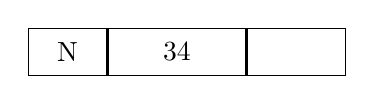
\begin{tikzpicture}
            % Define cell dimensions
            \def\cellone{1cm}
            \def\celltwo{1.75cm}
            \def\cellthree{1.25cm}
            \def\cellheight{0.6cm}
            % First cell with @ symbol
            \node[draw, rectangle, minimum width=\cellone, minimum height=\cellheight] (cell1) at (0,0) {\ml{N}};
            % Second cell positioned relative to the east edge of cell1
            \node[draw, rectangle, minimum width=\celltwo, minimum height=\cellheight, anchor=west] (cell2) at (cell1.east) {\ml{34}};
            % Third cell positioned relative to the east edge of cell2
            \node[draw, rectangle, minimum width=\cellthree, minimum height=\cellheight, anchor=west] (cell3) at (cell2.east) {};
        \end{tikzpicture}
        \\[18pt]
        %
        \raisebox{1.2cm}[0pt]{\shortstack[l]{Built-in\\ function}} &
        \raisebox{1.4cm}[0pt]{\ml{$+$}}
        &
        \begin{tikzpicture}
            % Define cell dimensions
            \def\cellone{1cm}
            \def\celltwo{1.75cm}
            \def\cellthree{1.25cm}
            \def\cellheight{0.6cm}
            % First cell with @ symbol
            \node[draw, rectangle, minimum width=\cellone, minimum height=\cellheight] (cell1) at (0,0) {\ml{P}};
            % Second cell positioned relative to the east edge of cell1
            \node[draw, rectangle, minimum width=\celltwo, minimum height=\cellheight, anchor=west] (cell2) at (cell1.east) {\ml{+}};
            % Third cell positioned relative to the east edge of cell2
            \node[draw, rectangle, minimum width=\cellthree, minimum height=\cellheight, anchor=west] (cell3) at (cell2.east) {};
            % Word below first cell
            \node (c) at ([xshift=0.5cm]cell1.center |- 0,-1.2) {Cell tag};
            % Letter x below third cell
%            \node (x) at (cell3.center |- 0,-1.2) {\ml{y}};
            % Arrow from second cell to f
            \draw[-{Stealth[length=3mm,width=2mm]}, thick] ([xshift=-0.5cm]c.north) -- (cell1.south);
            % Arrow from third cell to x
%            \draw[-{Stealth[length=3mm,width=2mm]}, thick] ([yshift=6pt]cell3.south) -- (x.north);
        \end{tikzpicture}
    \end{tabular}
}{Possible concrete representations}

\boxedfigure{
    \centering
    \begin{tikzpicture}
        % Define dimensions
        \def\cellwidth{0.8cm}
        \def\cellheight{0.6cm}
        \def\rowsep{1.4cm}
        \def\colsep{4cm}

        % Command to draw a row of three rectangles
        % Arguments: #1=anchor point, #2=row name prefix, #3,#4,#5=cell contents
        \newcommand{\drawrow}[5]{
            \node[draw, rectangle, minimum width=\cellwidth, minimum height=\cellheight] (#2cell1) at (#1) {#3};
            \node[draw, rectangle, minimum width=\cellwidth, minimum height=\cellheight, anchor=west] (#2cell2) at (#2cell1.east) {#4};
            \node[draw, rectangle, minimum width=\cellwidth, minimum height=\cellheight, anchor=west] (#2cell3) at (#2cell2.east) {#5};
        }

        % Draw the rows
        % Top row, left column
        \drawrow{0,0}{r1}{\ml{@}}{}{};

        % Top row, right column
        \drawrow{\colsep,0}{r2}{\ml{N}}{\ml{2}}{};

        % Middle row, left column
        \drawrow{0,-\rowsep}{r3}{\ml{@}}{}{};

        % Middle row, right column
        \drawrow{\colsep,-\rowsep}{r4}{\ml{N}}{\ml{4}}{};

        % Bottom row, left column
        \drawrow{0,-2*\rowsep}{r5}{\ml{P}}{\ml{+}}{};

        % Draw horizontal arrows from left column to right column
        \draw[-{Stealth[length=3mm,width=2mm]}, thick] (r1cell3.center) -- (r2cell1.west);
        \draw[-{Stealth[length=3mm,width=2mm]}, thick] (r3cell3.center) -- (r4cell1.west);

        % Draw vertical arrows connecting left column rows
        \draw[-{Stealth[length=3mm,width=2mm]}, thick] ([yshift=5pt]r1cell2.south) -- ++(0,-0.5) -| (r3cell1.north);
        \draw[-{Stealth[length=3mm,width=2mm]}, thick] ([yshift=5pt]r3cell2.south) -- ++(0,-0.5) -| (r5cell1.north);

        % Add the legend text
        \node[anchor=west] at (\colsep-.7cm,-2*\rowsep + 8pt) {
            \renewcommand{\arraystretch}{0.8}
            \begin{tabular}{l@{\hspace{4pt}}l@{\hspace{2pt}}l}
                Tags: & \ml{@} &application \\
                & \ml{P} &built-in \\
                & \ml{N} &number
            \end{tabular}
        };

    \end{tikzpicture}
}
{The concrete tree of \ml{(+ 4 2)}}


If the implementation supports variable-sized cells then we can implement
these structures directly:
\begin{center}
    {%
        \setlength{\tabcolsep}{12pt}
        \renewcommand{\arraystretch}{1.5}
        \sffamily
        \footnotesize
        \begin{tikzpicture}
            % Define dimensions
            \def\cellwidth{1.5cm}
            \def\cellheight{0.8cm}

            % Tag cell
            \node[draw, rectangle, minimum width=\cellwidth, minimum height=\cellheight] (tag) at (0,0) {Tag};

            % Field 1 cell
            \node[draw, rectangle, minimum width=\cellwidth, minimum height=\cellheight, anchor=west] (field1) at (tag.east) {Field 1};


            % Field n cell (positioned further right)
            \node[draw, rectangle, minimum width=\cellwidth, minimum height=\cellheight] (fieldn) at ([xshift=2.4cm]field1.east) {Field n};

            % Dots indicating more fields (automatically centered)
            \node at ($(field1.east)!0.5!(fieldn.west)$) {$\cdots$};
            \node at ($(field1.east)!0.5!(fieldn.west) + (0,0.3)$) {$\cdots$};
            \node at ($(field1.east)!0.5!(fieldn.west) + (0,-0.3)$) {$\cdots$};

            % Short lines extending from top and bottom borders
            \draw ([yshift=\cellheight/2]field1.east) -- ++(0.2,0);
            \draw ([yshift=-\cellheight/2]field1.east) -- ++(0.2,0);
            \draw ([yshift=\cellheight/2,xshift=-0.2cm]fieldn.west) -- ++(0.2,0);
            \draw ([yshift=-\cellheight/2,xshift=-0.2cm]fieldn.west) -- ++(0.2,0);

        \end{tikzpicture}
    }%
\end{center}

If the implementation supports fixed-size cells only, with two fields, then
the structure will have to be implemented as a linked collection of cells:
\begin{center}
    {%
        \setlength{\tabcolsep}{12pt}
        \renewcommand{\arraystretch}{1.5}
        \sffamily
        \footnotesize
        \begin{tikzpicture}
            % Define dimensions
            \def\cellwidth{1.5cm}
            \def\cellheight{0.7cm}
            \def\rowsep{1.25cm}

            % First row
            \node[draw, rectangle, minimum width=\cellwidth, minimum height=\cellheight] (r1tag) at (0,0) {Tag};
            \node[draw, rectangle, minimum width=\cellwidth, minimum height=\cellheight, anchor=west] (r1field1) at (r1tag.east) {Field 1};
            \node[draw, rectangle, minimum width=\cellwidth, minimum height=\cellheight, anchor=west] (r1field2) at (r1field1.east) {};

            % Second row
            \node[draw, rectangle, minimum width=\cellwidth, minimum height=\cellheight] (r2tag) at (0,-1.25*\rowsep) {Tag};
            \node[draw, rectangle, minimum width=\cellwidth, minimum height=\cellheight, anchor=west] (r2field1) at (r2tag.east) {Field 2};
            \node[draw, rectangle, minimum width=\cellwidth, minimum height=\cellheight, anchor=west] (r2field2) at (r2field1.east) {};

            % Third row
            \node[draw, rectangle, minimum width=\cellwidth, minimum height=\cellheight] (r3tag) at (0,-2.75*\rowsep) {Tag};
            \node[draw, rectangle, minimum width=\cellwidth, minimum height=\cellheight, anchor=west] (r3field1) at (r3tag.east) {Field n-1};
            \node[draw, rectangle, minimum width=\cellwidth, minimum height=\cellheight, anchor=west] (r3field2) at (r3field1.east) {Field n};

            % Arrows from first row to second row
            \draw[-{Stealth[length=3mm,width=2mm]}] ([yshift=8pt]r1field2.south) -- ++ (0, -20pt) -| (r2tag.north);

            % Dots between second and third row
            \node at ($(r2field2.center)!0.5!(r3field2.center) + (-2pt,3pt)$) {$\cdots$};
            % \node at ($(r2field2.center)!0.5!(r3field2.center)$) {$\vdots$};
            \node at ($(r2field2.center)!0.5!(r3field2.center) + (-2pt,9pt)$) {$\cdots$};

            % Arrow from second row area to third row
            \draw ([yshift=8pt]r2field2.south) -- ++ (0, -12pt) ;
            \draw[-{Stealth[length=3mm,width=2mm]}] ([yshift=-16pt]r2field2.south) -- ++ (0, -4pt) -| (r3tag.north);

        \end{tikzpicture}
    }%
\end{center}
Notice that, since the size of the structured object is determined by the
structure tag, the last cell can contain the last \textit{two} fields.

\subsection{Other Uses for Variable-sized Cells}

As we have seen, the provision of variable-sized cells gives a much more
efficient representation of structured data objects. However, variable-sized
cells may also be useful to contain other objects such as:
\begin{numbered}
    \item arrays;
    \item arbitrary precision integers;
    \item blocks of compiled code;
    \item multiple applications; for example, we could represent \ml{(f a b)} as a single
    three-field cell containing \ml{f}, \ml{a} and \ml{b}. This takes less space than the normal
    method, which requires two two-field cells.
\end{numbered}
Unfortunately, variable-sized cells carry an implementation cost, as we will
see in Chapter 17.

\section{Tags and Type-checking}

In what follows we will find it convenient to distinguish two families of tags.
The \textit{structure tags} identify data objects, and distinguish them from one
another. For example, a \ml{CONS} cell and \ml{NIL} would have distinct structure tags.
\textit{System tags} identify cells holding \textit{system objects}, such as application nodes,
lambda abstractions, built-in operators, and so on. The `\ldots\ and so on' is
highly implementation-dependent. For example, some implementations may
tag an application node differently if it is discovered to be irreducible, so that
repeated efforts to reduce it can be avoided.

\section{Compile-time versus Run-time Typing}

Some functional languages are polymorphically typed (see Chapter~8), and
type-checked at compile-time. In this case, only enough distinct tags are
required to identify system objects uniquely and to distinguish data objects of
a given type from each other (e.g.\ to distinguish a \ml{CONS} cell from \ml{NIL}). Thus
relatively few distinct tags are required, and a tag is typically represented in
eight bits or fewer.

Other languages rely on run-time type-checking, where each built-in
operator checks the type of its arguments before proceeding. This requires
that each data type be distinguishable from all the others used in the program.
Such run-time type-checked languages normally have only a fixed set of types,
and do not allow the user to introduce new types, so a fixed-size tag is still
sufficient.

Even in a type-checked system it is often considered desirable to carry
around type information at run-time to aid in system debugging. This is
problematic in languages that allow the programmer to introduce new types,
because there is no bound to the number of types which have to be distin-
guishable. In this case an escape mechanism is normally used for user-defined
types, whereby the first field of the cell representing the object carries a
unique type identification.

\section{Boxed and Unboxed Objects}

In Figure~10.4 each number seems to require a cell to itself. This seems rather
profligate, since a field of a cell is normally large enough to contain a number.
Thus, instead of a field pointing to a cell which contains a number, it would be
better to put the number directly in the field. For example, the tree repre-
senting \ml{(+ 4 2)} using unboxed representations would look like Figure~10.5
(compare Figure~10.4).

Data objects which can be completely described by a \textit{single field} are called
\textit{unboxed}, while those which are represented by \textit{one or more cells} are called
\textit{boxed} (the cell `boxes' the data object). Typical candidates for an unboxed
representation are integers, booleans, characters and built-in operators
(which can be identified by a small integer or code pointer). For example,
Figure~10.4 incorporates boxed representations of integers and built-in
functions, while Figure~10.5 gives them unboxed representations. It is clear
that significant savings in the number of cells allocated can be achieved by
using unboxed representations.

\begin{figure}[H]
    \centering

    {%
        \setlength{\fboxrule}{1pt}%
        \setlength{\fboxsep}{10pt}%
        \fbox{%
            \begin{minipage}{3cm}
                \centering
                \small
                \setlength{\parindent}{10pt}
                \setlength{\parskip}{0mm plus 0mm minus 0mm}
                    \vspace{-5pt}
                    \begin{tikzpicture}
                        % Define dimensions
                        \def\cellwidth{0.8cm}
                        \def\cellheight{0.6cm}
                        \def\rowsep{1.4cm}
                        \def\colsep{4cm}

                        % Command to draw a row of three rectangles
                        % Arguments: #1=anchor point, #2=row name prefix, #3,#4,#5=cell contents
                        \newcommand{\drawrow}[5]{
                            \node[draw, rectangle, minimum width=\cellwidth, minimum height=\cellheight] (#2cell1) at (#1) {#3};
                            \node[draw, rectangle, minimum width=\cellwidth, minimum height=\cellheight, anchor=west] (#2cell2) at (#2cell1.east) {#4};
                            \node[draw, rectangle, minimum width=\cellwidth, minimum height=\cellheight, anchor=west] (#2cell3) at (#2cell2.east) {#5};
                        }

                        % Draw the rows
                        % Top row
                        \drawrow{0,0}{r1}{\ml{@}}{}{\ml{2}};

                        % Bottom row
                        \drawrow{0,-\rowsep}{r3}{\ml{@}}{\ml{+}}{\ml{4}};

                        % Draw vertical arrows connectingrows
                        \draw[-{Stealth[length=3mm,width=2mm]}, thick] ([yshift=5pt]r1cell2.south) -- ++(0,-0.5) -| (r3cell1.north);
                    \end{tikzpicture}
                    \vspace{-5pt}
            \end{minipage}%
        }%
    }%

    \caption{\textsf The concrete tree of \ml{(+ 4 2)} (unboxed representations)}
\end{figure}

In a boxed system, the tag of a cell completely determines which fields of
the cell are pointers and which are not; for example, the two fields of an
application cell are always pointers (see Figure~10.4).

In contrast, in an unboxed system, any field which may contain a pointer
may also contain an unboxed object. For example, a field of an application cell
may either be a pointer or an unboxed (i.e.\ non-pointer) object (see Figure~10.5).
Hence, all such fields must have an extra bit, called the \textit{pointer-bit}, to
distinguish pointers from unboxed objects. Fields now look like this:

{%
%    \footnotesize
    \begin{tabular}{l@{\hspace{16pt}}l}
        A pointer field: &
        \begin{tikzpicture}
            \sffamily \footnotesize
            \node[draw, rectangle, minimum width=0.8cm, minimum height=0.6cm] (bit) {1};
            \node[draw, rectangle, minimum width=3.5cm, minimum height=0.6cm, anchor=west] (addr) at (bit.east) {Address\phantom{XXXX}};

            \node (pointer) at ([xshift=18pt]bit.center |- 0,1cm) {{\normalfont Pointer-bit}};
            % Vertical arrow from label to bit cell
            \draw[-{Stealth[length=3mm,width=2mm]}, thick] ([xshift=-18pt]pointer.south) -- (bit.north);
            % Arrow for address
            \draw[-{Stealth[length=3mm,width=2mm]}, thick] ([xshift=-0.5cm]addr.east) -- ++(2,0);
        \end{tikzpicture}
        \\[10pt]
        A non-pointer field: &
        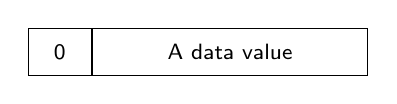
\begin{tikzpicture}
            \sffamily \footnotesize
            \node[draw, rectangle, minimum width=0.8cm, minimum height=0.6cm] (bit) {0};
            \node[draw, rectangle, minimum width=3.5cm, minimum height=0.6cm, anchor=west] (val) at (bit.east) {A data value};
        \end{tikzpicture}
    \end{tabular}
}%
\vs

A minor shortcoming of unboxed objects for run-time type-checked
systems is that unboxed objects are not tagged (since tags are attached to cells
not fields). In Figure~10.4, the \ml{N} tag on numbers enables the \ml{+} built-in
operator to check that its arguments are indeed numbers, whereas this is not
possible with a basic unboxed system. However, an unboxed system can still
incorporate run-time type-checking by reducing the number of bits in the
unboxed object sufficiently to fit a tag into the field as well. Non-pointer fields
would then look like this:
\begin{center}
    {%
        \sffamily \footnotesize
        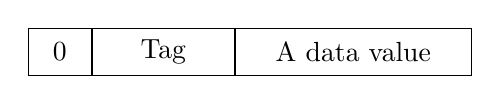
\begin{tikzpicture}
            \node[draw, rectangle, minimum width=0.8cm, minimum height=0.6cm] (bit) {0};
            \node[draw, rectangle, minimum width=1.8cm, minimum height=0.6cm, anchor=west] (tag) at (bit.east) {Tag};
            \node[draw, rectangle, minimum width=3cm, minimum height=0.6cm, anchor=west] (val) at (tag.east) {A data value};
        \end{tikzpicture}
    }%
\end{center}

Even for compile-time type-checked systems it is vital that built-in
functions (such as \ml{+}) are able to distinguish evaluated operands from
unevaluated ones (so that an unevaluated operand can first be evaluated).
Fortunately this is easy because if the operand is a pointer the tag on the cell
pointed to will show whether it is evaluated or not; and if the operand is a
non-pointer then it is an unboxed object which requires no further evaluation.

\section{Tagged Pointers}

Some implementations put a tag into pointer fields also, thus

\begin{center}
    {%
        \sffamily \footnotesize
        \begin{tikzpicture}
            \node[draw, rectangle, minimum width=0.8cm, minimum height=0.6cm] (bit) {1};
            \node[draw, rectangle, minimum width=1.8cm, minimum height=0.6cm, anchor=west] (tag) at (bit.east) {Tag};
            \node[draw, rectangle, minimum width=3cm, minimum height=0.6cm, anchor=west] (addr) at (tag.east) {Address\phantom{XX}};
            % Arrow for address
            \draw[-{Stealth[length=3mm,width=2mm]}, thick] ([xshift=-0.75cm]addr.east) -- ++(2,0);
        \end{tikzpicture}
    }%
\end{center}
For example, both the SKIM [Clarke \textit{et al.}, 1980] and NORMA [Richards,
1985] reduction machines do this, though they use the tag in different ways.
NORMA regards the pointer tag as a \textit{cache} for the tag of the cell pointed to.
Thus if the pointer tag is valid (one value of the pointer tag is reserved for
\ml{INVALID}) it contains the tag of the cell to which the pointer points. Like any
cache, this technique should be regarded purely as an optimization of the
ordinary tagged-cell approach.

In SKIM, however, there are no tags on cells at all. The only tags are in the
fields. This has the advantage that a cell now consists of two identical fields
(instead of two identical fields plus a tag), which allows a more uniform
hardware design for SKIM. However, it means that a cell cannot change its
tag; for example, an application cell must remain an application cell, because
it would be impossible to change the tags of all pointers to the cell at once.
This makes reduction slightly more awkward.

In summary, both a pure tagged cell and a pure tagged pointer approach
can adequately support reduction. The tagged cell approach makes reduction
rather easier, but gives rise to a rather less uniform hardware implementation.
The NORMA cacheing approach is more complex still, but may give some
performance improvement.

\section{Storage Management and the Need for Garbage Collection}

As reduction proceeds we will need to build new pieces of graph. In order to
do so we have to \textit{allocate} new cells. Cells are allocated from a (large) area of
storage called the \textit{heap}, which is simply an unordered collection of cells. The
term `heap' emphasizes that the physical adjacency of two cells is purely
coincidental; what matters is which cells point to which.

As well as allocating new cells, the reduction process will also discard cells,
or rather it will discard pointers to cells. We must re-use cells whenever
possible, because if we never did so we would soon run out of heap space.
Unfortunately, in a graph there may be many pointers to the same cell, and we
can only re-use a cell when there are no further pointers to it. So long as there
are further pointers to a cell from elsewhere in the graph, it cannot be re-used
because it is still in use. Cells with no pointers to them are said to be \textit{garbage}.
It is quite tricky to identify garbage cells, and all implementations of
functional languages include a \textit{garbage collector} whose purpose is to identify
and recycle garbage cells.

The whole activity of cell allocation and garbage collection is called storage
management, and is further discussed in Chapter~17. As we will see there,
fixed-size cells allow for a rather more simple garbage collector than variable-sized cells.

\section*{References}

\begin{references}

    \item Clarke, T.J.W., Gladstone, P.J.S., Maclean, C., and Norman, A.C. 1980. SKIM --
    The SKI reduction machine. \textit{Proceedings of the ACM Lisp Conference, Stanford, Calif.} 95044.

    \item Richards, H. 1985. \textit{An Overview of Burroughs NORMA}. Austin Research Center,
    Burroughs Corp., Austin, Texas. January.

\end{references}